\documentclass[11pt,a4paper]{article}

%%Packages needed in your paper

\usepackage[latin1]{inputenc}
\usepackage{amsmath}
\usepackage{amsfonts}
\usepackage{amssymb}
\usepackage{graphicx}
\usepackage{indentfirst}
\usepackage{setspace}
\usepackage{tikz}


%% The following are the page set-up
\setlength{\oddsidemargin}{-0.2in}
\setlength{\evensidemargin}{0.4in}
\setlength{\textwidth}{6.5in}
\setlength{\topmargin}{-1in}
\setlength{\textheight}{12in}

%% Enter the details of your paper

\author{Camille Shanes S. Fernandez}
\title{Research about Finding a New Family of Graceful Trees}


\begin{document}

%below starts your paper
\doublespacing
\newpage
\maketitle
\setlength{\parindent}{1cm} 
\begin{center}
	{\bf\ Review of Related Literature}
\end{center}

 \begin{enumerate}
%11
\item {\bfseries Olive Trees}\\
    An Olive tree is formed by attaching paths of consecutive lengths in a single vertex. Shown below is an example 
	\\
	\begin{center}
	\resizebox {0.3\textwidth} {0.7\height} {
		\begin{tikzpicture}[shorten >=2pt, auto, node distance=1cm,
		node_style/.style={circle,draw=black,fill=white!0!,font=\sffamily},
		edge_style/.style={draw=black}]
		
		\node[node_style] (n15) at (3,3)  {15};
		\node[node_style] (n12) at (5,2)  {12};
		\node[node_style] (n5) at (4.5,0.5)  {5};
		\node[node_style] (n9) at (4.5,-1)  {9};
		\node[node_style] (n6) at (3.5,0)  {6};
		\node[node_style] (n8) at (3.5,-1.5)  {8};
		\node[node_style] (n7) at (3.5,-3)  {7};
		\node[node_style] (n10) at (1,0)  {10};
		\node[node_style] (n4) at (1,-1.5)  {4};
		\node[node_style] (n11) at (1,-3)  {11};
		\node[node_style] (n3) at (1,-4.5)  {3};
		\node[node_style] (n0) at (-0.5,1)  {0};
		\node[node_style] (n14) at (-0.5,-1.5)  {14};
		\node[node_style] (n1) at (-0.5,-3)  {1};
	    \node[node_style] (n13) at (-0.5,-4.5)  {13};
		\node[node_style] (n2) at (-0.5,-6)  {2};
		
		\draw[edge_style]  (n15) edge node{3} (n12);
    	\draw[edge_style]  (n15) edge node{10} (n5);
    	\draw[edge_style]  (n5) edge node{4} (n9);
    	\draw[edge_style]  (n15) edge node{9} (n6);
    	\draw[edge_style]  (n6) edge node{2} (n8);
    	\draw[edge_style]  (n8) edge node{1} (n7);
    	\draw[edge_style]  (n15) edge node{5} (n10);
    	\draw[edge_style]  (n10) edge node{6} (n4);
    	\draw[edge_style]  (n4) edge node{7} (n11);
    	\draw[edge_style]  (n11) edge node{8} (n3);
    	\draw[edge_style]  (n15) edge node{15} (n0);
    	\draw[edge_style]  (n0) edge node{14} (n14);
    	\draw[edge_style]  (n14) edge node{13} (n1);
    	\draw[edge_style]  (n1) edge node{12} (n13);
    	\draw[edge_style]  (n13) edge node{11} (n2);
    
		\end{tikzpicture}}
		\begin{center}
		    Figure "insert number": A graceful olive tree
		\end{center}
		
\end{center}

    Dr. Jean Loyola discovered three new families of graceful trees.
%12	
\item {\bfseries $J_n$ Trees}\\
    $J_n$ trees are constructed by planting an end vertex of a path of length $i$, for $i=0,1,2,...,n-1$, in a parent path $v_0 v_1 v_2...v_{n-1}$ with a length of $n-1$. Shown below is an example of a graceful $J_4$ tree.
    \\
\newpage
	\begin{center}
	\resizebox {0.3\textwidth} {0.7\height} {
		\begin{tikzpicture}[shorten >=2pt, auto, node distance=1cm,
		node_style/.style={circle,draw=black,fill=white!0!,font=\sffamily},
		edge_style/.style={draw=black}]
		
		\node[node_style] (n0) at (0,0)  {0};
		\node[node_style] (n9) at (2,0)  {9};
		\node[node_style] (n2) at (4,0)  {2};
		\node[node_style] (n6) at (6,0)  {6};
		\node[node_style] (n1) at (2,2)  {1};
		\node[node_style] (n8) at (4,2)  {8};
		\node[node_style] (n3) at (4,4)  {3};
		\node[node_style] (n5) at (6,2)  {5};
		\node[node_style] (n7) at (6,4)  {7};
		\node[node_style] (n4) at (6,6)  {4};
		
		
		\draw[edge_style]  (n0) edge node{9} (n9);
    	\draw[edge_style]  (n9) edge node{7} (n2);
    	\draw[edge_style]  (n2) edge node{4} (n6);
    	\draw[edge_style]  (n9) edge node{8} (n1);
    	\draw[edge_style]  (n2) edge node{6} (n8);
    	\draw[edge_style]  (n8) edge node{5} (n3);
    	\draw[edge_style]  (n6) edge node{1} (n5);
    	\draw[edge_style]  (n5) edge node{2} (n7);
    	\draw[edge_style]  (n7) edge node{3} (n4);
		\end{tikzpicture}}
		
	
		
\end{center}
%13	
\item {\bfseries $J_{n,m}$ Trees}\\
    A $J_{n,m}$ tree is formed by taking $m$ copies of the $J_n$ tree and making the classification $v_{0,i}=v_{0,j}$ for all $0 {\geq} i$, $j {\geq} m$, provided that $m,n {\geq} 2$.Shown below is an example of a graceful $J_{3,3}$ tree.
	\\
	\begin{center}
	\resizebox {0.5\textwidth} {0.7\height} {
		\begin{tikzpicture}[shorten >=2pt, auto, node distance=1cm,
		node_style/.style={circle,draw=black,fill=white!0!,font=\sffamily},
		edge_style/.style={draw=black}]
		
		\node[node_style] (n0) at (3,0)  {0};
		\node[node_style] (n15) at (5,1)  {15};
		\node[node_style] (n10) at (1,1)  {10};
		\node[node_style] (n5) at (3,-2)  {5};
		\node[node_style] (n12) at (3,-4)  {12};
		\node[node_style] (n11) at (1,-2)  {11};
		\node[node_style] (n4) at (1,-4)  {4};
		\node[node_style] (n13) at (-1,-4)  {5};
		\node[node_style] (n7) at (-1,2)  {7};
		\node[node_style] (n6) at (3,2)  {6};
		\node[node_style] (n1) at (7,0)  {1};
		\node[node_style] (n2) at (7,2)  {2};
		\node[node_style] (n14) at (9,1)  {14};
		\node[node_style] (n3) at (11,0)  {3};
		\node[node_style] (n9) at (1,3)  {9};
		\node[node_style] (n8) at (3,4)  {8};
		
		\draw[edge_style]  (n0) edge node{10} (n10);
    	\draw[edge_style]  (n10) edge node{3} (n7);
    	\draw[edge_style]  (n7) edge node{2} (n9);
    	\draw[edge_style]  (n9) edge node{1} (n8);
    	\draw[edge_style]  (n10) edge node{4} (n6);
    	\draw[edge_style]  (n0) edge node{15} (n15);
    	\draw[edge_style]  (n15) edge node{14} (n1);
    	\draw[edge_style]  (n15) edge node{13} (n2);
    	\draw[edge_style]  (n2) edge node{12} (n14);
        \draw[edge_style]  (n14) edge node{11} (n3);
        \draw[edge_style]  (n0) edge node{5} (n5);
    	\draw[edge_style]  (n5) edge node{6} (n11);
    	\draw[edge_style]  (n5) edge node{7} (n12);
    	\draw[edge_style]  (n12) edge node{8} (n4);
        \draw[edge_style]  (n13) edge node{9} (n4);
    
		\end{tikzpicture}}
		
		
		
\end{center}

%14
\item {\bfseries $J_n$ + $J_{n+1}$ Trees}\\

    \indent 
    A  $J_n$ + $J_{n+1}$ tree is formed considering  $J_n$ and $J_{n+1}$ and making the identification
   
    $v_{i,n}=v_{i+n,n+1}$ for all $1\leq i\leq n-1$.Shown below is an example of a graceful $J_2$ + $J_3$ tree.
	\\
	\begin{center}
	\resizebox {0.3\textwidth} {0.7\height} {
		\begin{tikzpicture}[shorten >=2pt, auto, node distance=1cm,
		node_style/.style={circle,draw=black,fill=white!0!,font=\sffamily},
		edge_style/.style={draw=black}]
		
		\node[node_style] (n5) at (0,0)  {5};
		\node[node_style] (n2) at (2,0)  {2};
		\node[node_style] (n4) at (4,0)  {4};
		\node[node_style] (n3) at (6,0)  {3};
		\node[node_style] (n6) at (2,2)  {6};
		\node[node_style] (n0) at (2,4)  {0};
		\node[node_style] (n1) at (4,2)  {1};
	
		
		\draw[edge_style]  (n5) edge node{3} (n2);
    	\draw[edge_style]  (n2) edge node{2} (n4);
    	\draw[edge_style]  (n4) edge node{1} (n3);
    	\draw[edge_style]  (n2) edge node{4} (n6);
    	\draw[edge_style]  (n0) edge node{6} (n6);
    	\draw[edge_style]  (n6) edge node{5} (n1);
    
    
		\end{tikzpicture}}
		
		
\end{center}

%15
\newpage
Castilan and Zarraga discover three new familes of graceful trees namely, $\overline{P}_{(0,1)_n}(f)$,  $\overline{P}_{(0,2)_n}(f)$, and  $\overline{P}_{(0,3)_n}(f)$
\item {\bfseries $\overline{P}_{(0,1)_n}(f)$ Trees}\\
    % NEEDS DEFINITION
    Let $f(i)=k$ if $n=2k-1$ or $n=2k$. Let  $\overline{P}_{(0,1)_n}(f)=v_0 v_1 v_2\dots v_n$ be a path of length $n$ where $n$ is an even integer. Let $\overline{P}_{(0,1)_n}(f)$ be the tree obtained by planting an end vertex of a path $\overline{P}_i$ of length $f(i)$ to each $v_i$ for $i=1,2,\dots,n$. Shown below is an example of a graceful $\overline{P}_{(0,1)_4}(f)$ tree.
	\\
	\begin{center}
	\resizebox {0.4\textwidth} {0.7\height} {
		\begin{tikzpicture}[shorten >=2pt, auto, node distance=1cm,
		node_style/.style={circle,draw=black,fill=white!0!,font=\sffamily},
		edge_style/.style={draw=black}]
		
		\node[node_style] (n0) at (0,0)  {0};
		\node[node_style] (n10) at (2,0)  {10};
		\node[node_style] (n1) at (2,2)  {1};
		\node[node_style] (n2) at (4,0)  {2};
		\node[node_style] (n9) at (4,2)  {9};
		\node[node_style] (n8) at (6,0)  {8};
		\node[node_style] (n3) at (6,2)  {3};
	    \node[node_style] (n7) at (6,4)  {7};
		\node[node_style] (n5) at (8,0)  {5};
		\node[node_style] (n6) at (8,2)  {6};
		\node[node_style] (n4) at (8,4)  {4};
		
		\draw[edge_style]  (n0) edge node{10} (n10);
    	\draw[edge_style]  (n10) edge node{9} (n1);
    	\draw[edge_style]  (n10) edge node{8} (n2);
    	\draw[edge_style]  (n2) edge node{7} (n9);
    	\draw[edge_style]  (n2) edge node{6} (n8);
    	\draw[edge_style]  (n8) edge node{3} (n5);
        \draw[edge_style]  (n8) edge node{5} (n3);
    	\draw[edge_style]  (n3) edge node{4} (n7);
    	\draw[edge_style]  (n5) edge node{1} (n6);
    	\draw[edge_style]  (n6) edge node{2} (n4);
    
		\end{tikzpicture}}

\end{center}

%16 
\item {\bfseries $\overline{P}_{(0,2)_n}(f)$ Trees}\\

    Let $f(i)=k+1$ if $n=2k-1$ or $n=2k$, $k\geq1$. Let $\overline{P}_{(0,2)_n}(f)=v_0 v_1 v_2\dots v_n$ be a path of length $n$ where $n$ is an even integer. Let $\overline{P}_{(0,2)_n}(f)$ be the tree obtained by planting an end vertex of a path $\overline{P}_i$ of length $f(i)$ to each $v_i$ for $i=1,2,\dots,n$. Shown below is an example of a graceful $\overline{P}_{(0,2)_4}(f)$ tree.
	\\
	\begin{center}
	\resizebox {0.4\textwidth} {0.7\height} {
		\begin{tikzpicture}[shorten >=2pt, auto, node distance=1cm,
		node_style/.style={circle,draw=black,fill=white!0!,font=\sffamily},
		edge_style/.style={draw=black}]
		
		\node[node_style] (n0) at (0,0)  {0};
		\node[node_style] (n14) at (2,0)  {14};
		\node[node_style] (n1) at (2,2)  {1};
		\node[node_style] (n13) at (2,4)  {13};
		\node[node_style] (n3) at (4,0)  {3};
		\node[node_style] (n12) at (4,2)  {12};
		\node[node_style] (n2) at (4,4)  {2};
	    \node[node_style] (n11) at (6,0)  {11};
		\node[node_style] (n4) at (6,2)  {4};
		\node[node_style] (n10) at (6,4)  {10};
		\node[node_style] (n5) at (6,6)  {5};
		\node[node_style] (n7) at (8,0)  {7};
		\node[node_style] (n8) at (8,2)  {8};
		\node[node_style] (n6) at (8,4)  {6};
		\node[node_style] (n9) at (8,6)  {9};
		
		
		\draw[edge_style]  (n0) edge node{14} (n14);
    	\draw[edge_style]  (n14) edge node{13} (n1);
    	\draw[edge_style]  (n1) edge node{12} (n13);
    	\draw[edge_style]  (n14) edge node{11} (n3);
    	\draw[edge_style]  (n3) edge node{9} (n12);
    	\draw[edge_style]  (n12) edge node{10} (n2);
        \draw[edge_style]  (n3) edge node{8} (n11);
    	\draw[edge_style]  (n11) edge node{7} (n4);
    	\draw[edge_style]  (n4) edge node{6} (n10);
    	\draw[edge_style]  (n10) edge node{5} (n5);
    	\draw[edge_style]  (n11) edge node{3} (n7);
    	\draw[edge_style]  (n7) edge node{1} (n8);
    	\draw[edge_style]  (n8) edge node{2} (n6);
    	\draw[edge_style]  (n6) edge node{3} (n9);
    
		\end{tikzpicture}}

\end{center}

%17 
\item {\bfseries $\overline{P}_{(0,3)_n}$ $(f)$ Trees}\\

     Let $f(i)=k+2$ if $n=2k-1$ or $n=2k$, $k\geq1$. Let $\overline{P}_{(0,3)_n}(f)=v_0 v_1 v_2\dots v_n$ be a path of length $n$ where $n$ is an even integer. Let $\overline{P}_{(0,3)_n}(f)$ be the tree obtained by planting an end vertex of a path $\overline{P}_i$ of length $f(i)$ to each $v_i$ for $i=1,2,\dots,n$.Shown below is an example of a graceful $\overline{P}_{(0,3)_4}(f)$ tree.
	\\
	\begin{center}
	\resizebox {0.4\textwidth} {0.7\height} {
		\begin{tikzpicture}[shorten >=2pt, auto, node distance=1cm,
		node_style/.style={circle,draw=black,fill=white!0!,font=\sffamily},
		edge_style/.style={draw=black}]
		
		\node[node_style] (n0) at (0,0)  {0};
		\node[node_style] (n18) at (2,0)  {18};
		\node[node_style] (n1) at (2,2)  {1};
		\node[node_style] (n17) at (2,4)  {17};
		\node[node_style] (n2) at (2,6)  {2};
		\node[node_style] (n4) at (4,0)  {4};
		\node[node_style] (n15) at (4,2)  {15};
	    \node[node_style] (n3) at (4,4)  {3};
		\node[node_style] (n16) at (4,6)  {16};
		\node[node_style] (n14) at (6,0)  {14};
		\node[node_style] (n5) at (6,2)  {5};
		\node[node_style] (n13) at (6,4)  {13};
		\node[node_style] (n6) at (6,6)  {6};
		\node[node_style] (n12) at (6,8)  {12};
		\node[node_style] (n9) at (8,0)  {9};
		\node[node_style] (n10) at (8,2)  {10};
		\node[node_style] (n8) at (8,4)  {8};
		\node[node_style] (n11) at (8,6)  {11};
		\node[node_style] (n7) at (8,8)  {7};
		
		
		\draw[edge_style]  (n0) edge node{18} (n18);
    	\draw[edge_style]  (n18) edge node{17} (n1);
    	\draw[edge_style]  (n1) edge node{16} (n17);
    	\draw[edge_style]  (n17) edge node{15} (n2);
    	\draw[edge_style]  (n18) edge node{14} (n4);
    	\draw[edge_style]  (n4) edge node{11} (n15);
        \draw[edge_style]  (n15) edge node{12} (n3);
    	\draw[edge_style]  (n3) edge node{13} (n16);
    	\draw[edge_style]  (n4) edge node{10} (n14);
    	\draw[edge_style]  (n14) edge node{9} (n5);
    	\draw[edge_style]  (n5) edge node{8} (n13);
    	\draw[edge_style]  (n13) edge node{7} (n6);
    	\draw[edge_style]  (n6) edge node{6} (n12);
    	\draw[edge_style]  (n14) edge node{5} (n9);
    	\draw[edge_style]  (n9) edge node{1} (n10);
    	\draw[edge_style]  (n10) edge node{2} (n8);
    	\draw[edge_style]  (n8) edge node{3} (n11);
    	\draw[edge_style]  (n11) edge node{4} (n7);
    
		\end{tikzpicture}}
\end{center}

%18 

Manalo and Rosales generalized the three graceful trees found by Castilan and Zarraga and named the tree $P_{0,m_n} (f)$.
\item {\bfseries $P_{0,m_n}$ $(f)$ Trees}\\

    Let $f(i)=k+m-1$ if $i=2k-1$ or $i=2k$ where $k,m {\geq} 1$. Let $P_{0,m_n}$ $(f)$ tree be the tree obtained by considering a path $P_n = v_0 v_1 v_2...v_n$ of length $f(i)$ to each $v_i$ for $i=1,2,...,n$. 
	\\

%19 
Adaya and Crehencia discovered that all $P_{2n}(f)$ trees are graceful.
\item {\bfseries $P_{2n}(f)$ Trees}\\
    Let $f(n)=$
\begin{cases}
    0, \text{if $n$ is even}\\
    3, \text{if $n=4k-3$, $k \in \mathbb{N}$}\\
    5, \text{if $n=4k-1$, $k \in \mathbb{N}$}.
    
\end{cases}
\\
Let $P_{2n}(f)$ be the tree obtained by considering a path $P_{2n}=v_0 v_1 v_2\dots v_{2n}$ on $2n+1$ vertices and planting to $v_i$ an end vertex of the path $P_i$ of length $f(i)$ for $i=0,1,2,\dots,2n$.Shown below is an example of a graceful $P_8 (f)$ tree.
\newpage
	\begin{center}
	\resizebox {0.7\textwidth} {0.7\height} {
		\begin{tikzpicture}[shorten >=2pt, auto, node distance=1cm,
		node_style/.style={circle,draw=black,fill=white!0!,font=\sffamily},
		edge_style/.style={draw=black}]
		
		\node[node_style] (n0) at (0,0)  {0};
		\node[node_style] (n24) at (2,0)  {24};
		\node[node_style] (n2) at (2,2)  {2};
		\node[node_style] (n23) at (2,4)  {23};
		\node[node_style] (n3) at (2,6)  {3};
		\node[node_style] (n1) at (4,0)  {1};
		\node[node_style] (n20) at (6,0)  {20};
	    \node[node_style] (n6) at (6,2)  {6};
		\node[node_style] (n21) at (6,4)  {21};
		\node[node_style] (n5) at (6,6)  {5};
		\node[node_style] (n22) at (6,8)  {22};
		\node[node_style] (n4) at (6,10)  {4};
		\node[node_style] (n7) at (8,0)  {7};
		\node[node_style] (n19) at (10,0)  {19};
		\node[node_style] (n9) at (10,2)  {9};
		\node[node_style] (n18) at (10,4)  {18};
		\node[node_style] (n10) at (10,6)  {10};
		\node[node_style] (n8) at (12,0)  {8};
		\node[node_style] (n15) at (14,0)  {15};
		\node[node_style] (n13) at (14,2)  {13};
		\node[node_style] (n16) at (14,4)  {16};
		\node[node_style] (n12) at (14,6)  {12};
		\node[node_style] (n17) at (14,8)  {17};
		\node[node_style] (n11) at (14,10)  {11};
		\node[node_style] (n14) at (16,0)  {14};		
		
		\draw[edge_style]  (n0) edge node{24} (n24);
    	\draw[edge_style]  (n24) edge node{22} (n2);
    	\draw[edge_style]  (n2) edge node{21} (n23);
    	\draw[edge_style]  (n23) edge node{20} (n3);
    	\draw[edge_style]  (n24) edge node{23} (n1);
    	\draw[edge_style]  (n1) edge node{19} (n20);
        \draw[edge_style]  (n20) edge node{14} (n6);
    	\draw[edge_style]  (n6) edge node{15} (n21);
    	\draw[edge_style]  (n21) edge node{16} (n5);
    	\draw[edge_style]  (n5) edge node{17} (n22);
    	\draw[edge_style]  (n22) edge node{17} (n4);
    	\draw[edge_style]  (n20) edge node{13} (n7);
    	\draw[edge_style]  (n7) edge node{12} (n19);
    	\draw[edge_style]  (n19) edge node{10} (n9);
    	\draw[edge_style]  (n9) edge node{9} (n18);
    	\draw[edge_style]  (n18) edge node{8} (n10);
    	\draw[edge_style]  (n19) edge node{11} (n8);
    	\draw[edge_style]  (n8) edge node{7} (n15);
    	\draw[edge_style]  (n15) edge node{2} (n13);
    	\draw[edge_style]  (n13) edge node{3} (n16);
    	\draw[edge_style]  (n16) edge node{4} (n12);
    	\draw[edge_style]  (n12) edge node{5} (n17);
    	\draw[edge_style]  (n17) edge node{5} (n11);
    	\draw[edge_style]  (n15) edge node{1} (n14);
    	
		\end{tikzpicture}}

\end{center}

%20
Gonzales and Navarro found four new families of graceful trees namely, $M_n$, $Z_n$, $Z_n + Z_{n+1}$, and $O_n (1,3)$.
\item {\bfseries $M_n$ Trees}\\
    For $n\geq2$, let $M_n$ be the tree formed by considering a path $P_{2n+a}=v_0 v_1 v_2\dots v_2n$ on $n+1$ vertices and planting to $v_{2i-1}$ an end vertex of the path $P_i$ of length $i$, for $1=0,1,2,\dots,n$. Shown below is an example of grraceful $M_6$ tree.
	\\
	\begin{center}
	\resizebox {0.4\textwidth} {0.7\height} {
		\begin{tikzpicture}[shorten >=2pt, auto, node distance=1cm,
		node_style/.style={circle,draw=black,fill=white!0!,font=\sffamily},
		edge_style/.style={draw=black}]
		
		\node[node_style] (n0) at (0,0)  {0};
		\node[node_style] (n12) at (2,0)  {12};
		\node[node_style] (n2) at (2,2)  {2};
		\node[node_style] (n1) at (4,0)  {1};
		\node[node_style] (n10) at (6,0)  {10};
		\node[node_style] (n3) at (6,2)  {3};
		\node[node_style] (n11) at (6,4)  {11};
	    \node[node_style] (n4) at (8,0)  {4};
		\node[node_style] (n9) at (10,0)  {9};
		\node[node_style] (n6) at (10,2)  {6};
		\node[node_style] (n8) at (10,4)  {8};
		\node[node_style] (n7) at (10,6)  {7};
		\node[node_style] (n5) at (12,0)  {5};
		
		\draw[edge_style]  (n0) edge node{12} (n12);
    	\draw[edge_style]  (n12) edge node{10} (n2);
    	\draw[edge_style]  (n12) edge node{11} (n1);
    	\draw[edge_style]  (n1) edge node{9} (n10);
    	\draw[edge_style]  (n10) edge node{7} (n3);
    	\draw[edge_style]  (n3) edge node{8} (n11);
        \draw[edge_style]  (n10) edge node{6} (n4);
    	\draw[edge_style]  (n4) edge node{5} (n9);
    	\draw[edge_style]  (n9) edge node{3} (n6);
    	\draw[edge_style]  (n6) edge node{2} (n8);
    	\draw[edge_style]  (n8) edge node{1} (n7);
    	\draw[edge_style]  (n9) edge node{4} (n5);
    
		\end{tikzpicture}}
\end{center}
\end{enumerate}

       
\end{document}

